
\begin{frame}{Gráficos por Computadora}
%\begin{block}{Gráficos por Computadora} 
\begin{columns}
\begin{column}{0.58\textwidth}
    \begin{center}

\begin{itemize}
\item Es la rama de las CC encargada de la producción de imágenes y animaciones empleadas en juegos de computadora y simulaciones, en algunos casos incluyendo elementos fotorealisticos.
\item Se requieren conocimientos de geometría, algebra, cálculo, física, programación (estructura de datos). 
\item Existen liberias de bajo nivel (OpenGL) hasta frameworks (Unity, Unreal).
\end{itemize}
     \end{center}

\end{column}
\begin{column}{0.42\textwidth}  
    \begin{center}
     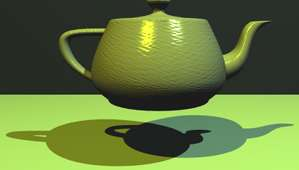
\includegraphics[width=0.9\textwidth]{Figs/GC1}\\
     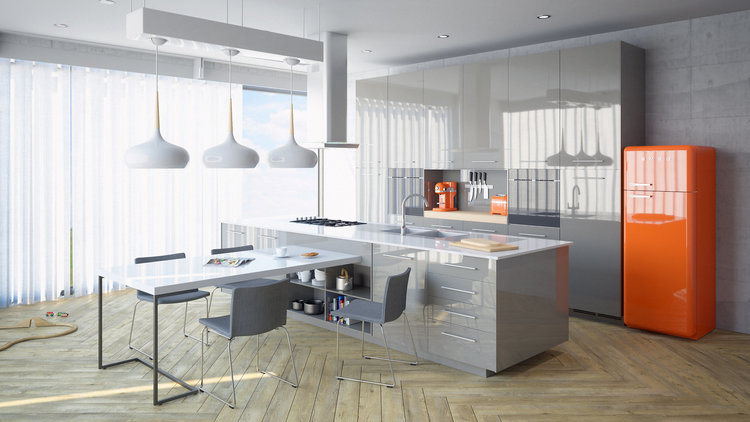
\includegraphics[width=0.9\textwidth]{Figs/GC2}\\
     \end{center}
\end{column}
\end{columns}
%\end{block} 
\end{frame}

